\chapter{State of the Art}
\section{Software defined networks}
In this section I will first try to define what a \gls{sdn} are. Then we will look at different components of an \gls{sdn} like the controller, the networking element and the different \gls{api}s.
\subsection{SDN terminology and definition}
\label{sec:sdn_definition}
If you read books or papers about \gls{sdn} you would most likely find many different flavor of a definition for \gls{sdn}. Some will define it as a framework \cite{SDN_Anatomy_of_OpenFlow}, other defines it as an architecture with a centalization of the control plane \cite{SDN_Comprehensive} \cite{foundations_2015}. Nevertheless, what they usually have in common is that they define \gls{sdn} to be a way to make networks programmable by separating the control and data plane and connecting them through well defined \gls{api}s\cite{SDN_Anatomy_of_OpenFlow}. Where the dataplane is the part of the network that forward data from one port to another based on the \gls{fib} or forwarding table and the control plane is the part of the network that make forwarding decision and populate the \gls{fib}. 
\par
I will use this definition through this thesis and I would also emphasize that the location of the control plane does not have to be a single centralized controller. There are many advantages by centralizing the control plane like faster response to link failure because the information does not have to propagate through multiple nodes, loop avoidance since the controller has the complete picture, added agility when there is only one controller to configure, increased reliability due to less direct human interaction and centralized policy enforcement \cite{SDN_Anatomy_of_OpenFlow}. The obvious drawbacks are a single point of failure and attack focus, scale and latency when updating the switch which can lead to temporarily microloops (also an issue in todays networks) \cite{SDN_Anatomy_of_OpenFlow}  \cite{SDN_Comprehensive, p 48}. In addition military networks are usually connected with radio links or even sattelite with high latency and low bandwidth which amplifies the drawbacks with a centralized controller. As we will see later in this thesis there has to be some sort of dynamic controll assignment so that the network can take advantage of centralized controller when it is in a stable state but also has some kind of mechanism to function autonomously when disconnected from the controller. 
\par
Figure \ref{fig:sdn_components} shows the components of a \gls{sdn}, with the data plane which resieds on a Network element, the control plane on the \gls{sdn} controller, the management plane which are annotated as applications or services and standardised \gls{api}s to communicate between these elements. The next few section would go more in details about these component. 


\begin{figure}
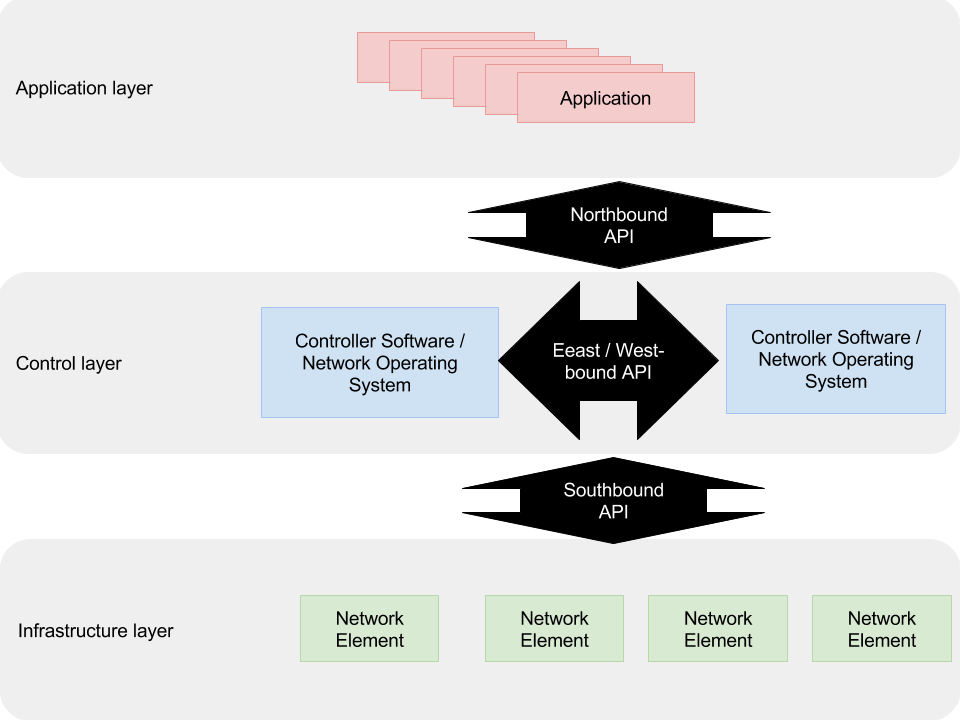
\includegraphics[width=5in]{content/img/sdn_components.png}
\caption{\gls{sdn} components}
\label{fig:sdn_components}
\end{figure} 


\subsection{Networking Element}
In traditional networks it is usual to distinguish between routers which operates on layer three and switches which operates on layer two,there are even a third class of devices known as L3 switches. The biggest difference between these devices lies in the control plane and how they get knowledge about the network and populate the \gls{fib}. When looking at the data plane all devices have the same mission - to forward data entring on one port to another port. In \gls{sdn} the control plane is logically separated from the physical data plane, hence all these devices are really just forwarding elements. 

\subsection{\gls{sdn} Controller}
======THIS SECTION HAS TO BE REWRITTEN========
The device that holds the controller logic a software defined network is often called a \gls{sdn} controller or a \gls{nos}. Many examples: OpenDaylight (open source controller) Floodlight, Cisco XNC, POX, NOX, ONOS, Beacon, Trema, Maestro, NodeFlow. There are huge differences between these controllers. Both regarding their \gls{api}s and what features they support.  


\subsection{XX-bound \gls{api}}
As mentioned in \ref{sec:sdn_definition} \gls{sdn} is about making networks programmable through well defined \gls{api}s. The purpose of an \gls{api} is to enable interaction between components, and . As figure \ref{fig:sdn_components} shows it is usual to categories the \gls{api}s in three different categories. The Southbound \gls{api} is the interface towards the networking element, and OpenFlow and Netconf are examples of open source Southbound \gls{api}s while OnePK is a Cisco propiritary protocol. The Northbound \gls{api} is the interface of the controller towards applications or services. These \gls{api} make some abstractions so the application should not have to care about the detailed configuration of the networking element. A often used Northbound \gls{api} are \gls{rest} \gls{api}. A \gls{rest} \gls{api} often communicates over HTTP and uses a standard representation format like \gls{json}, \gls{html} or \gls{xml}. Other Northbound \gls{api}s are programming languages like JAVA or propritary \gls{api}s. The East / Westbound \gls{api} are \gls{api}s to communicate between \gls{nos} or Controllers SDNi, BGP, AMQP.


\subsubsection{OpenFlow}
OF protocol, instruction set, architectue => interface\cite{sdn_Anatomy_of_OpenFlow} 

OF components:

\subsection{ONOS controller} 

\section{Distribution}
\subsection{Techniques}
\subsection{Leader Election}
\subsection{Synchronization}

\section{Federated Networks}
\subsection{Federated Mission Network}
\cite{http://www.act.nato.int/fmn}
\gls{fmn} and \gls{jmei}. Define number plans and protocols for how to connect to each nation. BGP, NTP, SNMP, ... Five service: Each nation has to manually configure their BGP peers before each . 

Four leel of capability, Mission Network Element (MNE), Mission Network eXtension (MNX) - self served but may not include sufficient mission essential services, Hosted User, other entities


FMN Affiliate : " NATO and Non-NATO nations are encouraged to become FMN Affiliates, which implies they will maintain and further develop capabilities for federated mission networks and ensure CIS security and interoperability compliance with FMN standards and principles. FMN Affiliates will be able to contribute FMN-ready forces to a mission on short notice and with minimal preparation."

\subsection{Protected Core Networks}
\section{TACOMS}
\section{TACOMS}
\gls{tacoms} was a multinational initiative with the goal to specify how \gls{nato} nations should connect in order to achieve interoperability in military operations on a tactical level. 
The next section will briefly take you through \gls{tacoms} more than 30 years of history, including the different versions of the framework called \gls{tacoms} phase 1, \gls{tacoms} phase 2 and \gls{tacoms}+. In the following sections the overall architecture of \gls{tacoms}+ will be explain together with a detailed description of the autoconfiguration specification for \gls{tacoms}+. The technical details for the other \gls{tacoms} specifications are not relevant in this thesis. I will conclude this section with my own thoughts regarding the design of \gls{tacoms} autoconfiguration specification including the advantages and weaknesses. 
\subsection{History}
\gls{tacoms} was established in 1985 as a multinational initiative by 12 \gls{nato} nations \footnote{Belgium, Canada, France, Germany, Italy, The Netherlands, Norway, Portugal, Spain, Turkey, United Kingdom and United States}. The nations saw the requirement for a new NATO standard for telecommunication due to the rising need for interoperability in the battlefield. \footnote{\gls{tacoms} were not restricted to NATO nations, but included Partnership for Peace nations. Sweden and Finland joined in 2007 when signing the 2nd \gls{mou}.} \footnote{Poland was part of \gls{tacoms} for a short period of time from 2003 to 2007 when the 2nd amendment of the \gls{mou} was signed.} \cite{https://www.tacoms.org/pages/history.aspx}. In June 2010 \gls{tacoms} phase 1  \gls{stanag}s (STANAG 4637 - 4647) were successfully promulgated as official \gls{nato} standards \cite{https://www.tacoms.org/pages/about.aspx}.The STANAG 4637-family define a protocol suite and addressing scheme for the physical layer up to the transport layer in the \gls{osi} model in addition it describe how \gls{voip} should be handled up to the application layer. However only the Netherlands implemented the STANAG 4637-family \gls{tacoms} in their tactical communication system. I think one reason for this was that some of the protocols were at the end-of-life when the STANAGs were finally finalized, like the H.323 signalling protocol which lost terrain against \gls{sip}. Another reason can be that \gls{nato} started their own standardization project for information sharing and interoperability namely the \gls{fmn}, which was based on the success and lessons learned from \gls{amn} \footnote{the operational NATO network in Afghanistan} \ref{sec:fmn}. . 

After completion of  the STANAGs in 2010, \gls{tacoms} continued as \gls{tacoms} phase 2 with a \gls{mou} / agreement ending in 2012. With phase 2, the first flavor of \gls{sdn} or programmable networking were introduced with the \gls{sow} 6 - Flexibility, Agility and Scalability \ref{sec:sow6}. Some nations withdraw from the project when entering phase 2, due to \gls{fmn} and other reasons (lost thrust because of the time it took for STANAG 4637 to come to life).  By end of the second \gls{mou}, \gls{tacoms} decided to change the strategy from writing STANAGs to rather contribute to the \gls{fmn} work. The same year \gls{tacoms} phase 1, with some quick wins (like replacing H.323 with SIP), was accepted as the transport layer for \gls{fmn}. The third \gls{mou} was signed and later extended until March 2016 in order to complete the work \footnote{Norway, Spain, Turkey, UK, Sweden, Finland, The Netherlands signed the extension. Italy withdraw, but participated in some of the work}. 

( 
Proof of concept at the \gls{cwix} exercise in 2015 in Bydgoszcz, Poland.
SDN track within FMN?
 
)

\gls{tacoms} work group finalized their work during March 2016. 

Lost many nations when they needed an extended MOU (Italy, Germany while Canada, USA exit earlier) 
 continued 2014-2016 

\subsection{TACOMS+ Technical}
\subsubsection{Architecture}
 %%%%%%EVERYTHING IS COPIED FROM TACOMS ARCHI%%%%%%
“While implementation of the UNI was national concern, implementation of NIP is coalition concern. Therefore, functions and protocols exchanged across the NIP are standardized in a detail.” 
“What does TACOMS+ provide?
TACOMS+ provides the standards that enable seamless interoperability at network domain between differing national networks to effectively create a single, coherent Mission Network. TACOMS+ creates the interface between national networks but does not impact on the national systems or capabilities. TACOMS+ utilises open standards and industry best practice to define the interoperability interfaces and the TACOMS+ standards provide the recommendations and approaches to be taken when implementing those protocols. TACOMS+ is therefore not a bespoke hardware solution, neither is it a system or a stand-alone item of equipment.”
\cite{tacoms_architecture_concept}

The different areas in TACOMS are covered by a number of profiles. Each profile is documented in one or more documents. The documents have been produced by sub teams of TACOMS, called Statement of Work (SoW), as an answer to the statement of need (SoN) decided by TACOMS PSG for each team.

Area
Profile
Documents
Technical specifications, implementation examples etc
Network Infrastructure/ Network services
Dual Stack
CL Forwarding Routing
Autoconnectivity
CL Forwarding Auto Connectivity
Bearers Transmission Mediation
(moved from CL Forwarding)
CO communication
CO Forwarding
Future bearers
Bearers -----
Voice


CO Forwarding
FMN Spiral 1 for Media
Addressing
Addressing
CL Forwarding -  Address and Numbering Plan
Network Support Services
Name Resolution
Network support services- Name Resolution
Time Synchronization
Network support services- Time Synchronization
Security
Border Protection System 
CL Forwarding Border Protection System
Public Key Infrastructure
Network support services- Public Key Infrastructure
Authentication
CL Forwarding Authentication

\gls{tacoms} includes two different automatic -> “autoconnectivity” and “service announcement”. Autoconnectivity includes discovery peers, mutual authentication and automatic peering of GRE tunnels, BGP routing and multicast routing. 

\subsubsection{Autoconnectivity}
\gls{tacoms} autoconnecitivity technical specification \cite{tacoms_t6_autoconf_techspec}
BGP, GRE, MSDP,
The entities are successfully authenticated with IKE over IPSEC. 
\gls{tacoms} autoconnectivity technical specification \cite{tacoms_t6_autoconf_techspec} divides the process for autoconfiguration in three phases: discovery, authentication and automated configuration of peers. Phase one and three rely on routing-protocols to share configuration information and a custom software to use this information to configure peers, while phase three rely on IKE over IPsec.


\subsubsubsection{Discovery}
PRECONFIGURATION:
The nodes are preconfigured with a 111.[Entity_number].x.y/8 IPv4. 
Used as source for RIPv2 packets and later as source / destination for the GRE tunnel between the nations. 
RIPv2 with
Pre-shared key and MD5 authentication
Announced 110.[Entity_number].x.y/32 address 
This network is not used for anything, only to announce the physical destination address of the GRE-tunnel (111./8 address). 

=> The Discovery phase is used to discover other \gls{tacoms} nation by announcing a /32 subnet with RIPv2. With the second octet identifying the entity it is possible to decide who would serve as a master and slave in the preceding steps. MD5 authentication with pre-shared key are used to reduce DoS attacks. 

With the extracted source of the RIPv2 announcement it is possible to start configuring a GRE tunnel with IPSEC adding the physical source and destination. The nation with the highest entity number serves as the master and start to configure the logical address of the tunnel. IPv6 is enabled at the tunnel endpoint which will enable RIPng packets to start flowing, hence phase two and autoconfiguration. 
 

The interface meant for \gls{tacoms} connectivity are configured with a  address where the second and this octet identify the nation.



The spec claims that - “This document uses the address plan designed by the SoW6-group. The discovery mechanism is not bound to that exact address plan, and can be adjusted to cohere with other address plans. When IPv6 becomes the dominant network layer technology, the entire address plan and the auto-discovery mechanisms should be updated to utilize new functionality in IPv6. “  however to identify a configuration announcement / service announcement feature it rely on the  on the script / nation software  



 \cite{tacoms_t6_autoconf_techspec}

\subsubsubsection{TACOMS Design choices}
\cite{T6-Concept_options} “...rationale for the design choices of TACOMS SON 6 group” = > Autconfiguration.
Authentication:
Options
X509v3 certificates 
Phase 1 Discovery Protocol:
Options
Custom protocol and mDNS = not part of COTS feature set. 
OSPF
RIPv2 
IPv6 Routing Protocols
Phase 2 Service Announcement Protocol
Options
Custom protocol
IPv4 Routing protocols
OSPF for IPv6
RIPng
Service Announcement
Options
DNS
UDDI
BGP



%%%%%%%%%%%%%%%Netconf survey START%%%%%%%%%%%%%%%%%
\cite{http://blog.ipspace.net/2015/10/survey-vendor-netconf-and-rest-api.html}
Routers
Vendor
NETCONF
Pure XML?
REST API
Alcatel Lucent
Yes


?
Brocade MLX
Yes


?
Cisco IOS / IOS XE
Yes
Some
No
Cisco CSR 1000V
Yes
Some
Yes (JSON)
Cisco IOS XR
Yes


?
Juniper
Yes
Yes
Yes
Updates:
IOS XR has NETCONF;
REST API is only available on CSR 1000V, not on IOS or IOS XE in general;
Juniper MX routers have REST API in Junos release 15.1;
Brocade MLX routers and ALU routers have NETCONF support;

%%%%%%%%%%%%%%%NETCONF Survey END%%%%%%%%%%%%%%%%%


---DRAW PROTOCOL in VSD----

RIPv2 - discovery (with pre-shared key)
RIPng - autconf (Over GRE tunnel 
GRE w/Ipsec - Authentication

\subsection{TACOMS+ Thoughts}
\subsubsection{Advantages}
Rely on existing standards
Except the software / script that are triggered by an autoconf event, all the code is configuration of existing standards
Introduces agility and flexibilty to FMN in a secure (?) manner
Tested 
Though at every exercise something failed

\subsubsection{Critique}
\gls{tacoms} autoconfiguration has a very “dirty” design, this is due to the inflexibility to future changes, mixing of concerns, highly coupled and dependent, duplication of functionality and lack of abstractions. 

%INFLEXIBLE%
\gls{tacoms} encapsulate information in IPv6 addresses to share configuration information,. An IPv6 address is 128 bits long, where the first 32 bits are used to identify the type of information being encapsulated. This leaves 96 bits for configuration information, and in most cases they use additional 16 or 32 bits to identify the entity sending the information. Even though \gls{tacoms} has proved that this information serves the purpose for configuring both \gls{gre}, \gls{msdp} and \gls{bgp}, it makes the protocol inflexible to future changes. What if \gls{fmn} decides to change the routing protocol? What if the length of the telephone number i changed, exceeding the length of an IPv6 address? With the method of encapsulation information in IPv6 addresses \gls{tacoms} makes the protocol inflexible to future changes in other part of the framework. (makes it also dependent upon IPv4 - how do you encapsulate a IPv6 within IPv6???). 
To make things happen faster they have to tweak the timers of the \gls{rip}, \gls{ripng} and \gls{bgp}.  = > Now 60 sec for peering. 
Dependent upon the addressing scheme

%MIXING OF CONCERNS%
\gls{bgp} is both used for announcing regular IPv6 routing information and \gls{tacoms} configuration information. The Service announcement routes are fake and not routable. \gls{tacoms} specify these routing processes to be separated, but this will actually in many cases mean an additional bgp router or software router (Cisco, as example, only support one bgp routing instance in each \gls{vrf}, and one tunnel can only have one \gls{vrf}...) %%%CHECK REF%%%%

%Dependencies%
\gls{tacoms} rely on \gls{rip} for discovery, \gls{ripng} for sharing peering information and \gls{bgp} for service announcement. Even though these protocol have been around for a while and would most likely not change in the future, it is not a good design principles to rely on these protocols.
Tacoms software would
Much static / pre-configuration that needs tweaking / workarounds of a regular router to work
Since there are so many protocols involved in the autoconfiguration process there is a need for a lot of preconfiguration/static of the IOP.
Some of the pre-configuration needs workarounds (eks when having more than one interface means having the same ip subnet for multiple interfaces on a router) because it is not standards procedure.
Injecting non-existing network addresses by adding loopback addresses. 

%Lack of abstractions and high coupling to the underlying HW%
Lack of abstraction => Not possible for a collaborative software development, and reuse of software. 
The implementation is highly dependent on the underlying HW / SW implementation. 

Many protocols used for other purposes than its original design
TACOMS uses RIPv2 for discovery, but it is not the announced address which is of interest but the source of the routing information. 
RIPng to share GRE tunnel address, Multicast information
link-by-link (not redistributed
BGP IPv6 for service annoucement (encoded by FD00:<serviceId>:<NationId>:<NationDomain>:)
TACOMS also specify regular IP v4/v6 forwarding with BGP and demands that the nation uses two different routing instances, one for forwarding and one for SA.
Not consistent - in some situation you only uses the announced ip address and other also the announced next-hop address.
Some are redistributed depending on the service ID.
=> Has to “inject” ipv4/ipv6 addresses that are not addressable
Latency of convergence because of timeout and trigger interval of the different protocols
Rely on pre-shared certificates
Maybe not possible to avoid if you will keep it secure
Error prone conversion of IPv6 addresses 
Both hex-bin, hex-decimal in the same operation
Depending of the prefix length and the announced service, what part of the address which are hex-bin and hex-dec are changes. 
Depends on the prefix mask and how the ipv6 address is represented (if aggregated with :: for 0000 for example)
Inconsistency of address allocation
Master node is the node with the largest entity number, and is the one deciding the interface addresses. 

BGP to share information. SOW6-8. Delivered the first STANAG TACOMS phase 1 in 2010. TACOMS+ next phase. Terminated March 2016. IPO opened in 1998 \cite{tacoms.org}.  8 Statement of Needs. Architecture, Phase 1 QuickWins, Reference implementation, Support to NATO FMN, Security, Agility and Flexibility, CO Services, Future IOP Bearers and Interfaces. Based on standard routing protocol to share information. RIP, RIPng and BGPv6. 
